\chapter{Testování}
%TODO vysledky zobrozene v TrackLabu !

%TODO mozna neco z testovani zaradit do sekce realizace. predevsim nejake promerovani parametru? a tady nechat jen zasadni info o dulezitych testech

\section{Napájení}
% TODO V2 uvest rozbehove sekvence celeho zarizeni  !!
% TODO V2 stailita 1V2ANA 1V2DIG pro Timepix2 !!
Na základní desce jsou generované celkem 3 napájecí úrovně z +5 V externího napájení USB, jak bylo uvedeno v sekci \ref{napajeni}. A to napájecí úrovně +1.2 V, +2.5 V a +3.3 V. Zvlnění výstupního napětí bylo poté vždy měřeno na výstupu každého spínaného regulátoru se snahou vytvoření co nejkratší zemní smyčky mezi měřícím bodem a připojenou zemí osciloskopu. Měření nebylo ve všech případech s ohledem na velikost zemní smyčky ideální vzhledem k zapojení ve kterém je realizováno vyčítací rozhraní a to tedy v zapojení, kdy je deska s Timepix 2 nad základní deskou a tedy není možné se připojit sondou osciloskopu na vrchní stranu základní desky. I s ohledem na zmíněné problémy byly naměřeny tyto průběhy \ref{fig:napeti}. Kde CH3 je +2.5 V, CH2 +3.3V a CH1 poté +1.2 V. Stejnosměrné hodnoty výše uvedených napájecích úrovní je možné vidět na obrázku \ref{fig:urovne}.
\begin{figure}[h!]
	\centering
	\captionsetup{justification=centering}
	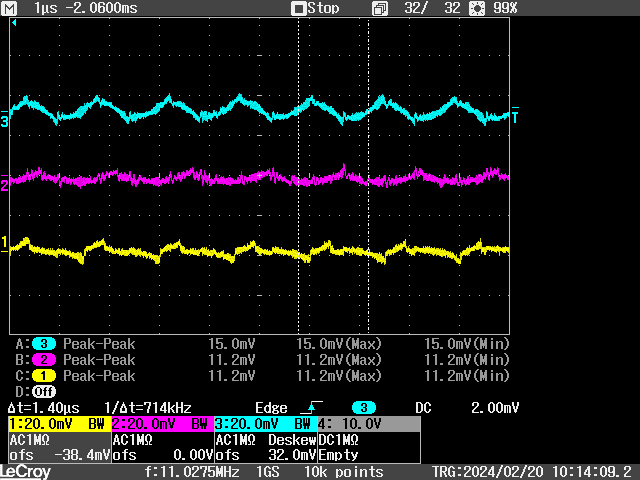
\includegraphics[scale=0.40]{./Mereni/ripple 3V3 - CH2 & 2V5 - CH3 & 1V2 - CH1, 2x 47uF.png}
	\caption{Zvlnění napětí výstupních napětí +2.5V, +3.3 V a +1.2 V } 
	\label{fig:napeti}
\end{figure}

\begin{figure}[h!]
	\centering
	\captionsetup{justification=centering}
	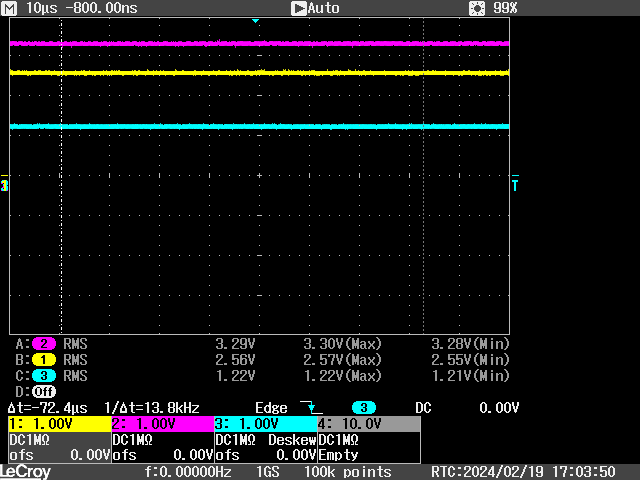
\includegraphics[scale=0.40]{./Mereni/vout 3V3 & 2V5 & 1V2.png}
	\caption{Stejnosměrné úrovně výstupních napětí, +2.5V, +3.3 V a +1.2 V, spínaných regulátorů na základní desce \ref{zakladni deska}} 
	\label{fig:urovne}
\end{figure}

\section{Integrace rozhraní do programu TrackLab}
Velkou část ověření funkčnosti navrženého rozhraní v této práci tvořila integrace rozhraní do programu TrackLab \cite{Manek_2024}. Tento program slouží pro zpracování dat z pixelových detektorů, online analýzu dat a automatizaci. Navržené rozhraní je připojeno pomocí virtuálního ethernetu pes USB do uživatelského rozhraní. Protokol, kterým rozhraní komunikuje je analogický, jako pro vyčítací rozhraní Katherine pro Timepix 2, které bylo popsáno v části \ref{Katherine}. Protokol je založen na 6 B rámcích, které jsou posílány pomocí UDP protokolu. Pokud nebude uvedeno jinak, pořízené snímky ověřující funkcionalitu rozhraní jsou z právě programu TrackLab \cite{Manek_2024}.

\begin{figure}[h!]
	\centering
	\captionsetup{justification=centering}
	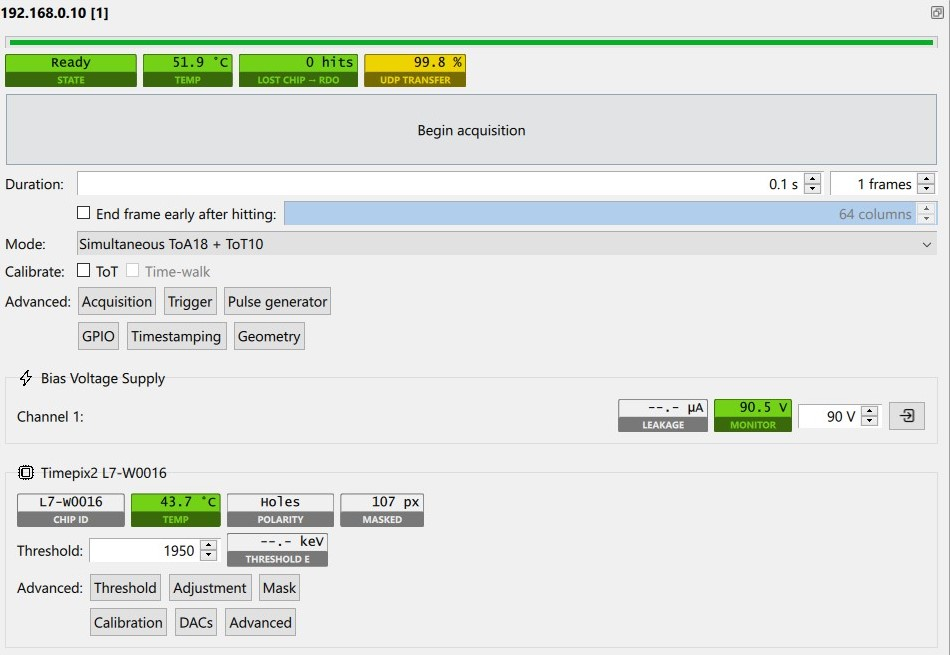
\includegraphics[scale=0.55]{tracklab_info.jpg}
	\caption{Hlavní panel programu TrackLab \cite{Manek_2024}} 
	\label{fig:Tracklab}
\end{figure}



\section{Vysokonapěťový zdroj}
% Nastaveni VN zdroje
Zapojení vysokonapěťového zdroje a princip měření vysokého napětí, které je generováno na desce s Timepix 2 \ref{Deska s Timepix2} je popsán v části textu \ref{VN zdroj}. Velikost vysokého napětí je nastavována přes SPI komunikaci z mikrokontroléru. Velikost výstupního napětí je poté možné nastavit v rozsahu 8-bitového čísla, tedy 256 hodnot. Závislost 8-bitové hodnoty na výstupním napětí vysokonapěťového zdroje je možné vidět na obrázku \ref{fig:hv_hex}, kdy nastavené vysoké napětí bylo zpětnovazebně měřeno mikrokontrolérem. Monitorované vysoké napětí je poté monitorováno programem TrackLab, jak lze vidět na obrázku \ref{fig:Tracklab}.
\begin{figure}[h!]
	\centering
	\captionsetup{justification=centering}
	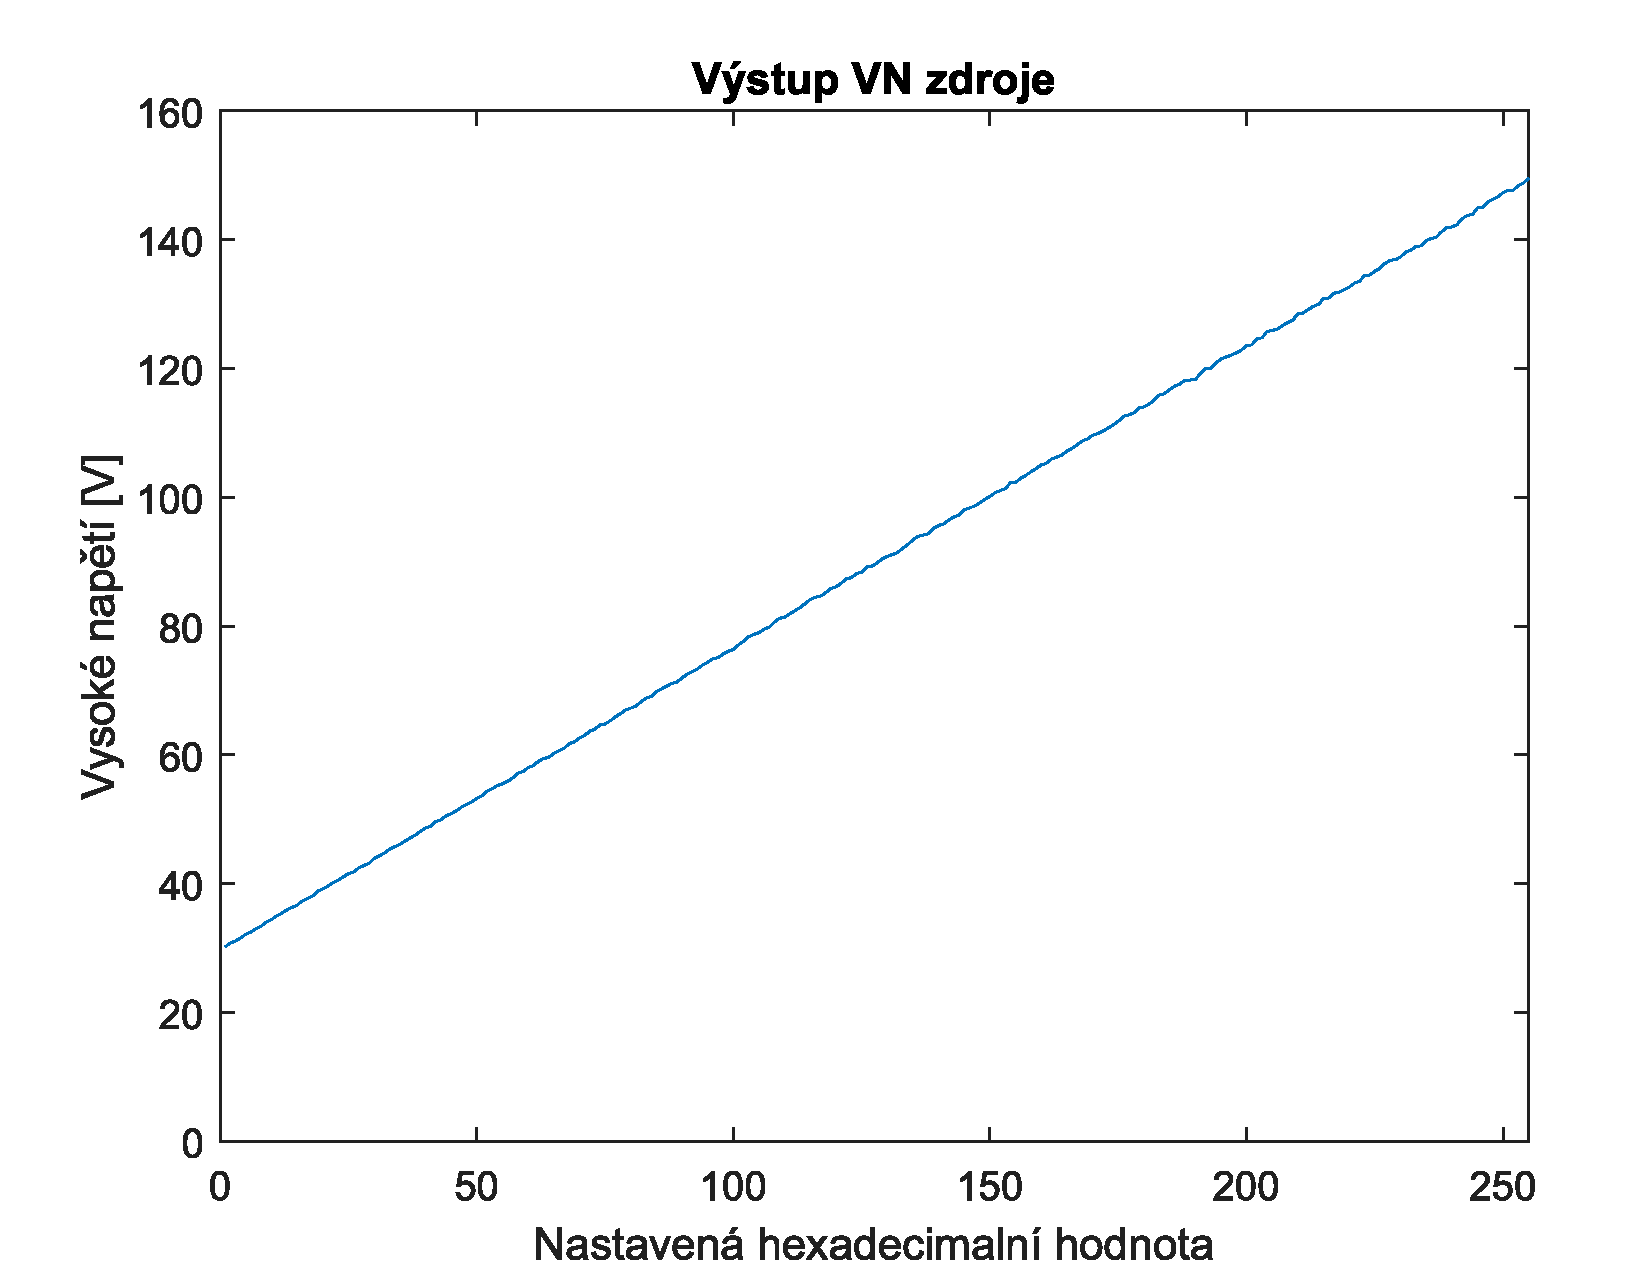
\includegraphics[scale=0.40]{./Mereni/hv_hex_small.pdf}
	\caption{Závislost vstupní 8 bitové hodnoty na výstupním napětí VN zdroje.} 
	\label{fig:hv_hex}
\end{figure}

% TODO promereni teploty s mechanikou ??, termokamra ??
\section{Měření teploty}
V této práci bylo implementováno měření teploty pomocí externího teplotního senzoru na desce s detektorem Timepix 2 \ref{Deska s Timepix2} a měření teploty za využití interního měření teploty detektoru Timepix 2.
\subsection{Měření teploty vyčítacího rozhraní}
Typ senzoru který byl pro tuto práci vybrán pro měření teploty na desce s Timepix 2 byl podrobně popsán v části \ref{Mereni teploty}. Pokud dojde k uživatelskému příkazu, který požaduje informaci o teplotě, následuje proces vyčtení teploty ze senzoru pomocí I2C komunikace. Poté následuje dekódování přijatého čísla na odpovídající skutečnou hodnotu. Zobrazení teploty na desce s detektorem Timepix 2 je poté monitorováno z programu TrackLab \cite{Manek_2024}. Zobrazení teploty lze vidět na obrázku \ref{fig:Tracklab}.
\subsection{Měření teploty Timepix2}
Pixelový detektor Timepix 2 umožňuje monitorovat vnitřní teplotu detektoru. Hodnota výsledné teploty detektoru je poté dle simulace teploty detektoru v závislosti na napěťové referenci popsána na obrázku \ref{fig:tpx2_temp}. Pro získání teploty detektoru je zapotřebí naměření dvou analogových hodnot z obrázku \ref{fig:tpx2_temp}, označovaných jako Vtemp a Vbg. Pro získání těchto analogových hodnot je nejprve zapotřebí nastavit, jaká hodnota analogového napětí bude na výstupu pinu Timepix 2 označovaného jako DACOUT. Výstup pinu DACOUT Timepix 2 je poté zpracován interním 12-bitovým AD převodníkem mikrokontroléru na základní desce \ref{zakladni deska}. Příklad výběru hodnoty na výstup DACOUT detektoru Timepix 2 a převod získaných hodnot na odpovídající teplotu lze vidět v \ref{kod_temp_tpx2}.
\begin{lstlisting}[frame=single, language=C, caption={Výběr výstupu DACOUT detektoru Timepix2 a odečtení hodnoty detektoru}, label=kod_temp_tpx2]
// GET DAC : VBG_TEMP
uint8_t set_dacoutsel[0] = VBG_TEMP; 
float vtemp = 0;
// set what type of DAC will be on DACOUT output								   
if(tpx2_set_reg_8b(TPXA, SET_DACOUTSEL, set_dacoutsel) != TPX_OK) {    
	Error_Handler();
}
if(board_tpx2_get_dacout(TPXA, &vtemp) != BOARD_OK) {
	Error_Handler();
}
// Sim. -> TT. // Temp. into real value in ^C.
float tpx2_temp = 471.99*(vtemp - vbg)/1000 - 179.14;					
\end{lstlisting}
Následně zpracovaná teplota je odeslána do programu TrackLab. Zobrazení teploty detektoru Timepix 2 lze najít na obrázku \ref{fig:Tracklab}.  
\begin{figure}[h!]
	\centering
	\captionsetup{justification=centering}
	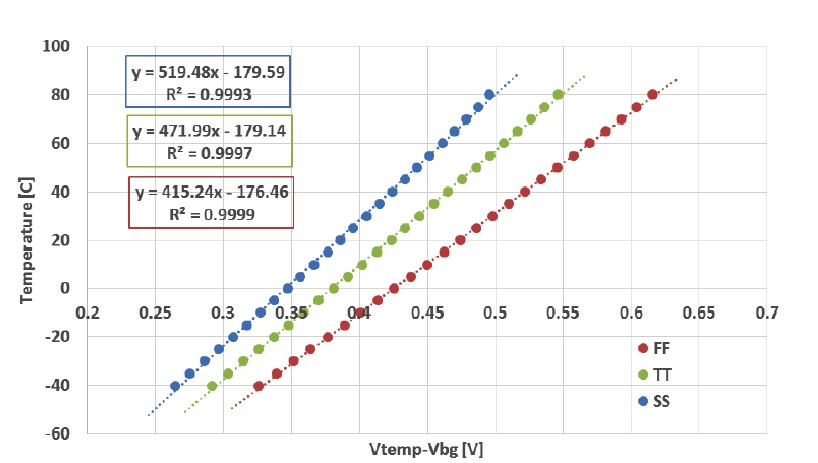
\includegraphics[scale=0.50]{tpx2_temp.jpg}
	\caption{Simulace teploty detektoru Timepix2 v závislosti na hodnotě napěťové reference \cite{tpx2_manual}.} 
	\label{fig:tpx2_temp}
\end{figure}

\section{Komunikační rozhraní s Timepix 2}		% promřování logických urovni komunkikace, rychlosti atd..
%todo logicke urovne SLVS, rychlosti komunikace -> need V2. MCLOCK..
Komunikační rozhraní detektoru Timepix 2 bylo popsáno v části textu \ref{Komunikacni rozhrani}. Následná  realizace komunikace s Timepix 2, pak v části \ref{CPLD konverze}. K měření diferenciálních komunikačních signálů byla použita aktivní diferenciální sonda s osciloskopem. Měření probíhalo při frekvenci komunikačních hodin 20 Mhz. Na obrázku \ref{fig:MCLOCK_DIFF_PROBE} můžete vidět průběh komunikačních hodin. Konkrétně CH 2 z obrázku \ref{fig:MCLOCK_DIFF_PROBE} je výstup hodinového signálu SPI komunikace z mikrokontroléru. Kanál CH 1 je poté naměřený diferenciální signál aktivní diferenciální sondou po konverzi logické úrovně v CPLD, který je poté na vstupu detektoru Timepix 2.  
\begin{figure}[h!]
	\centering
	\captionsetup{justification=centering}
	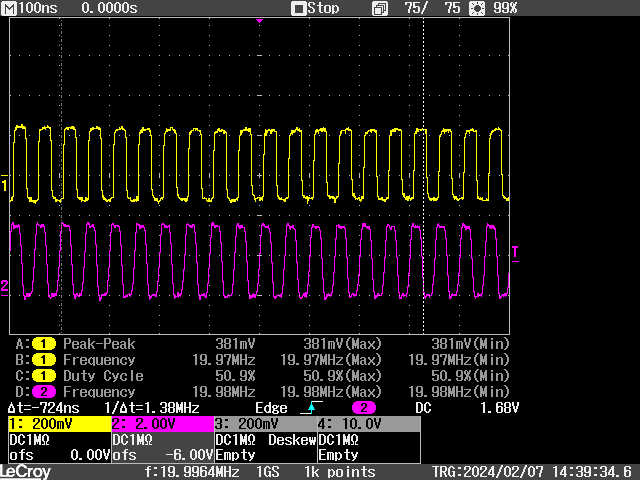
\includegraphics[scale=0.40]{./Mereni/MCLOCK_DIFF_PROBE.png}
	\caption{Průběh hodinového signálu pro komunikaci s Timepix 2} 
	\label{fig:MCLOCK_DIFF_PROBE}
\end{figure}

\section{Digitální test Timepix 2} %popis prubehu a vysledku
Funkčnost komunikace s detektorem Timepix 2 byla, také ověřena pomocí digitálních testů, jednotlivé testy budou popsány v následujících částech.
	\subsection{Vyčtení chip ID}
	Prvním digitálním testem, který byl implementován byl test, který vyčítá sériové výrobní číslo detektoru, označované jako CHIP ID, které je pro každý detektor Timepix 2 jedinečné a předem známé. Pro správné vyčtení CHIP ID detektoru je nejprve zapotřebí přivést napájecí napětí +2.5 V na pin VDD33, jak bylo popsáno v části \ref{Technicka specifikace}. Hodnota CHIP ID je poté uložena v 32-bitové registru Timepix 2. Vyčtením tohoto registru dostáváme 32 bitovou hodnotu, kterou pomocí známé transformace převedeme na skutečnou hodnotu CHIP ID, která odpovídá předem známému sériovému číslu detektoru Timepix 2. Program TrackLab, před každým připojením nového rozhraní vyčte sérové číslo připojeného detektoru. Výpis získaného CHIP ID v programu TrackLab lze vidět na obrázku \ref{fig:Tracklab}.

	\subsection{Vyčtení a zapsání pixelových matic}
	Pomocí výše uvedeného testu, vyčtení CHIP ID detektoru došlo k otestování vyčítaní základních registrů detektoru Timepix 2. Dalším digitálním testem je poté zápis a vyčtení všech čítačů, používajících se pro měření. Popis čítačů Timepix 2, lze najít v části \ref{Digitálni cast}.
	\par Zápis do digitálních čítačů slouží jen pro digitální testování, při samotném měření se tato funkce nevyužívá. S výjimkou nastavení konfigurační matice a matice lokálních prahových úrovní, které využívají pro nastavení 10-bitový a 4-bitový čítač. Celkem při digitálním testu došlo k zápisu hodnot do všech dostupných čítačů Timepix 2 a následnému vyčtení. Celkem bylo zapsáno 5 testujících obrazů. Zapsané obrazy byly zvoleny dle tabulky \ref{tab:obraz}. Při digitálním testu tedy došlo k zápisu 327 680B dat a jejich opětovnému vyčtení. Digitální test byl prováděn s frekvencí datových hodin 40 Mhz. Po každém digitálním testu bylo resetováno napájení detektoru Timepix 2 a digitální test byl proveden znovu. Při opakovaném digitálním testu, nebyly pozorovány problémy. %Test byl opakován 100 krát s úspěšností 100\%.
	\begin{table}[h!]
		\centering
		\begin{tabular}{ |P{3cm}|P{3cm}|  }
			\hline
			\multicolumn{2}{|c|}{Vybrané zapsané obrazce} \\
			\hline
			Test  & Obraz\\ \hline \hline 
			1 & 0xFF \\ \hline 	
			2 & 0x00 \\ \hline 		 
			3 & INC \\ \hline
			4 & DEC \\ \hline
			5 & 0xAA\\ \hline
		\end{tabular}
		\caption{Digitální test, zapisované hodnoty}
		\label{tab:obraz}
	\end{table}
\section{Timepix 2 DAC}
	Dalším testem ověřením funkčnosti navrženého vyčítacího rozhraní byl DAC sken Timepix 2. Test při kterém do 18 interních DAC kanálů detektoru Timepix 2 byla pro každý kanál zapsána digitální 8-bitová hodnota v rozsahu 0 až 255. Následně byl zvolen DAC kanál, který bude výstupem na pinu DACOUT detektoru Timepix 2. Tato již analogová hodnota z výstupního pinu DACOUT byla převedena interním 12-bitovým AD převodníkem mikrokontroléru. DAC sken pro 18 interních kanálů s výpisem do programu TrackLab můžete vidět na obrázku \ref{fig:dacscan}. 
	\begin{figure}[h!]
		\centering
		\captionsetup{justification=centering}
		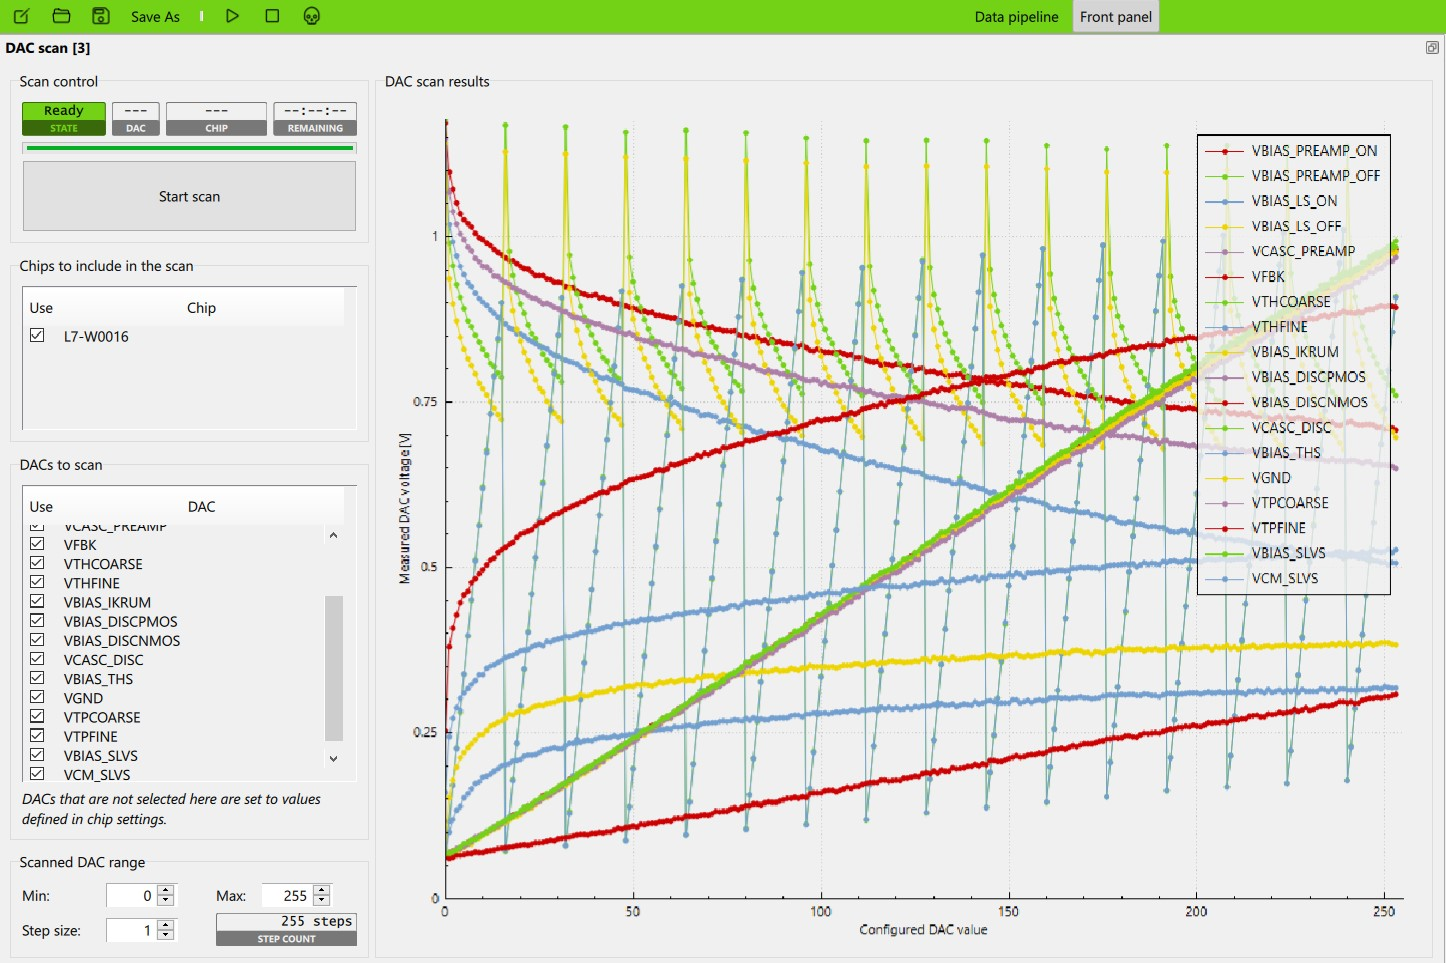
\includegraphics[scale=0.50]{tracklab_dac.jpg}
		\caption{DAC sken detektoru Timepix 2.} 
		\label{fig:dacscan}
	\end{figure}
\section{USB komunikace}
%todo, dokumentace funkčnosti... -> VCM, pak UDP pres USB
Fyzická implementace USB byla popsána v části textu \ref{USB}. Pro testování USB komunikace byly použity dvě USB třídy. První třídou USB byl virtuální sériový port přes USB. Druhou třídou byla pak třída RNDIS, neboli virtuální ethernet přes USB, jež byla použita pro přenos UDP protokolu přes USB.
\subsection{Virtuální ethernet přes USB}
	Další USB třídou, která byla použita v konečné implementaci byla třída RNDIS. Jedná se o třídu zařízení kdy je přes USB implementován virtuální ethernet. V této práci se konkrétně pomocí USB přenáší UDP protokol. Tato třída byla zvolena s ohledem na existující program TrackLab \cite{Manek_2024}. TrackLab umožňuje připojit různá vyčítací rozhraní s pixelovými detektory. Vyčítací rozhraní v této práci respektuje již existující standart a to standart připojení vyčítacího rozhraní Katherine pro Timepix 2 \ref{Katherine}. Ukázka nakonfigurovaného zařízení jako třídy RNDIS lze vidět na obrázku \ref{fig:RNDIS}. Snímek konfigurace zařízení byl pořízen z programu USBTreeView. 
	%TODO USB RNDIS konfigurace
	\begin{figure}[h!]
		\centering
		\captionsetup{justification=centering}
		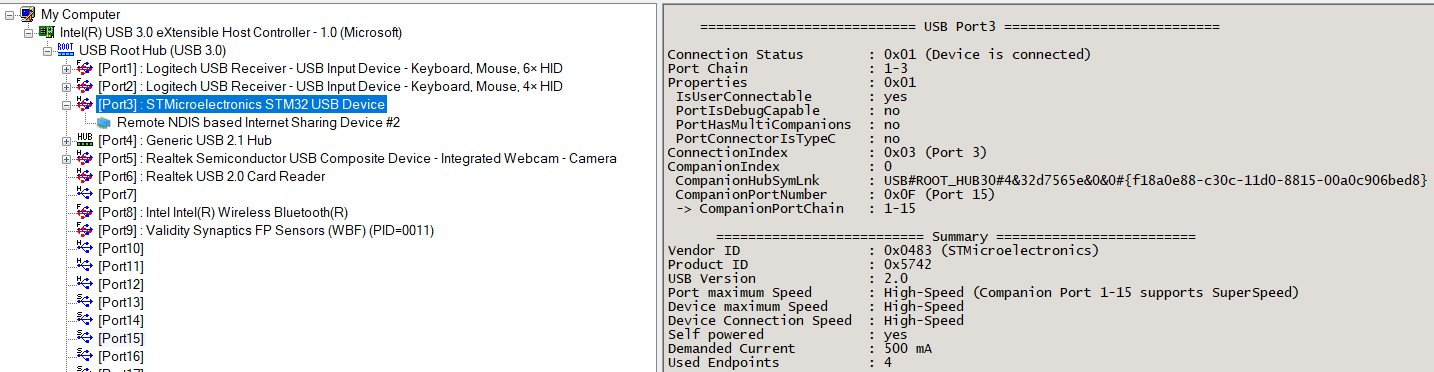
\includegraphics[scale=0.50]{usb_view.jpg}
		\caption{Vyčítací rozhraní nakonfigurované jako zařízení z USB třídy RNDIS.} 
		\label{fig:RNDIS}
	\end{figure}
%TODO mam dat zvlast tridu o TrackLabu?
	

\section{Měření spotřeby}
%todo spotreba, bez chipu, s chipem, zavislosti?

	
\section{Dosažené parametry}
% TODO shrnuti nosazenych parametru namerenych vyse


